\documentclass[12pt]{article}
\usepackage[utf8]{inputenc}
\usepackage[T1]{fontenc}
\usepackage{amsmath,amssymb,graphicx,geometry}
\geometry{margin=2.5cm}
\title{Calibração dos parâmetros $\beta$ e $\gamma$ no modelo SIR:\\ surto de influenza de 1978 -- ajuste usando somente a coluna $B$}
\author{}
\date{}
\begin{document}
\maketitle
\section{Objetivo}
Este texto descreve a calibração dos parâmetros $\beta$ e $\gamma$ do modelo SIR para o surto de influenza ocorrido em uma escola inglesa em janeiro--fevereiro de 1978. O ajuste é feito usando \emph{somente} os valores da coluna $B$ (``confined to bed''). A coluna $C$ não entra no funcional de mínimos quadrados.
\section{Dados}
A população total é $N=763$. Tomamos $t=0$ em 22 de janeiro de 1978. Os 14 valores da coluna $B$ são
\[
B=(3,8,26,76,225,298,258,253,189,128,68,29,14,4).
\]
\section{Interpretação de $B$}
No modelo SIR, $I(t)$ representa o número de indivíduos no compartimento infeccioso. A coluna $B$, porém, é uma categoria observacional: ``confined to bed''. Neste exercício fazemos a aproximação
\[
I_{\rm obs}(t_i)=B_i.
\]
Isto é uma hipótese de modelagem: $B$ não é necessariamente idêntico, em sentido epidemiológico estrito, ao compartimento infeccioso $I$.
\section{Modelo SIR}
\[
\frac{dS}{dt}=-\beta\frac{SI}{N},\qquad
\frac{dI}{dt}=\beta\frac{SI}{N}-\gamma I,\qquad
\frac{dR}{dt}=\gamma I.
\]
Com $S+I+R=N$ e condições iniciais
\[
(S(0),I(0),R(0))=(760,3,0).
\]
Os parâmetros têm unidade $\mathrm{dia}^{-1}$ e
\[
R_0=\frac{\beta}{\gamma},\qquad 1/\gamma
\]
é a duração média do estado infeccioso no modelo.
\section{Ajuste por mínimos quadrados}
Para cada $(\beta,\gamma)$ resolvemos o SIR e minimizamos
\[
\Phi(\beta,\gamma)=\sum_{i=0}^{13}[I(t_i;\beta,\gamma)-B_i]^2,
\qquad \beta,\gamma\geq0.
\]
Portanto, somente $B$ aparece no objetivo.
\section{Implementação em Python}
Usamos \texttt{odeint} para resolver as EDOs e \texttt{curve\_fit} para os mínimos quadrados não lineares:
\begin{verbatim}
def Icurve(tt,beta,gamma):
    return odeint(rhs,[760.,3.,0.],tt,
                  args=(beta,gamma))[:,1]

popt,_=curve_fit(Icurve,t,B,p0=(1.5,.3),
                 bounds=(0,np.inf),maxfev=20000)
\end{verbatim}
\section{Resultado numérico}
O ajuste usando somente $B$ fornece
\[
\boxed{\widehat\beta=1.68875843\ \mathrm{dia}^{-1}},
\qquad
\boxed{\widehat\gamma=0.44011957\ \mathrm{dia}^{-1}}.
\]
Logo,
\[
\boxed{\widehat R_0=3.83704459},
\qquad
\boxed{1/\widehat\gamma=2.27210981\ \mathrm{dias}}.
\]
O erro quadrático residual e o RMSE são
\[
\mathrm{RSS}=4593.93932508,
\qquad
\mathrm{RMSE}=18.11459421.
\]
\section{Gráfico}
\begin{center}
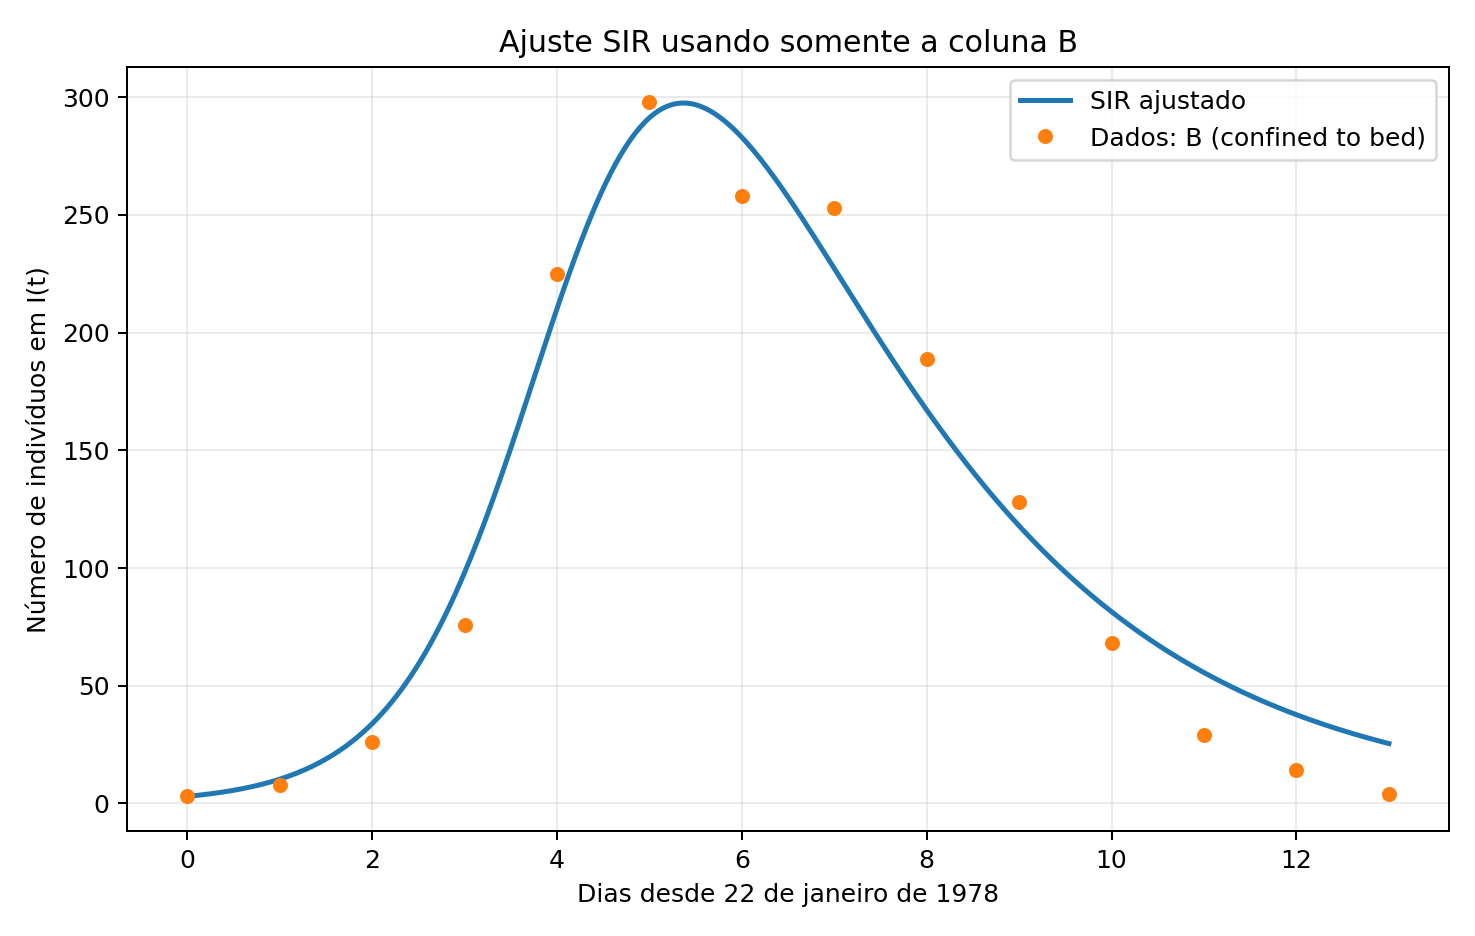
\includegraphics[width=0.90\textwidth]{calibracao_SIR_surto_BMJ_White_coluna_B.png}
\end{center}
\section{Comparação com o ajuste usando $B+C$}
No ajuste anterior, usando $I_{\rm obs}=B+C$, obtiveram-se aproximadamente
\[
\widehat\beta=1.440772,\qquad \widehat\gamma=0.263430,
\qquad \widehat R_0=5.469282.
\]
Os dois problemas não são o mesmo: aqui a variável observada é somente $B$. A diferença mostra a sensibilidade dos parâmetros estimados à definição da variável identificada com $I$.
\section{Comparação com White}
Na discussão associada ao exemplo, White apresenta valores de referência aproximadamente
\[
\beta=1.97\ \mathrm{dia}^{-1},\qquad \gamma=0.47\ \mathrm{dia}^{-1},\qquad R_0\approx4.18.
\]
Uma reprodução numérica simples não precisa coincidir exatamente: podem influir a escolha da variável observada, as condições iniciais, o funcional de erro, o intervalo de ajuste, arredondamentos e detalhes do procedimento original.
\section{Reprodução}
Instale:
\begin{verbatim}
pip install numpy scipy matplotlib
\end{verbatim}
e execute:
\begin{verbatim}
python calibracao_SIR_surto_BMJ_White_coluna_B.py
\end{verbatim}
\section{Referências}
\begin{enumerate}
\item ``Influenza in a boarding school'', \emph{British Medical Journal}, 1978.
\item P. J. White, discussão de modelos matemáticos em epidemiologia, incluindo o exemplo do surto de influenza e a Fig.~5-2.
\item G. De Vries et al., \emph{A Course in Mathematical Biology}, SIAM, 2006.
\item P. Virtanen et al., ``SciPy 1.0: Fundamental Algorithms for Scientific Computing in Python'', \emph{Nature Methods} 17 (2020), 261--272.
\item J. Nocedal and S. J. Wright, \emph{Numerical Optimization}, 2nd ed., Springer, 2006.
\end{enumerate}
\end{document}
